\section{Event simulation}
\label{sec:larsoftsim}

Two kinds of events must be simulated in the ProtoDUNE-SP detector
geometry: beam events and cosmic-ray events.  Beam events are
generated using a dedicated particle gun generator that has as input
parameterizations of the flux and the beam profile parameters.
Upstream beam instrumentation devices, such as wire chambers,
Cherenkov counters, and time-of-flight counters are also to be
simulated but as of this writing are not yet included.  Cosmic-ray
events are simulated either with the CRY~\cite{cry} event generator or
the CORSIKA~\cite{corsika}.  Neutrino scattering events are simulated
using GENIE~\cite{genie}.  While neutrino scattering events are likely
to be rare in protoDUNE-SP, the extrapolation of the performance of
the detector to the FD may require simulating neutrino scattering
events protoDUNE-SP.  A dedicated generator in LArSoft simulates
radionuclide decay products which can be overlaid on other events.

The detector geometry is coded in GDML files~\cite{geant4} that are
generated by the gegede~\cite{gegede} geometry system.  These files
contain the locations, sizes, shapes, and material content of the
detector components, the active liquid argon volume, and the
surrounding materials, such as the field cage, the beam windows, the
cryostat the supporting structure, and the experimental hall.  These
external features will impact the distributions of cosmic-ray
particles impinging on the active detector.  The channels and volumes
are numbered and named in the GDML files, with conventions followed by
the LArSoft simulation code.

The active volume of the detector is divided into cubes 300~$\mu$m on
a side, called voxels.  GEANT4 tracks particles through the argon, and
each step ends on a voxel, allowing precise simulation of small-scale
physics processes such as delta-ray emission and showering at a level
of detail smaller than the intrinsic resolution of the detector.  The
simulation of the ionization and scintillation photon emission from
the steps is done either with a dedicated parameterization that
depends on the electric field in the liquid argon and the ionization
density~\cite{birks}, or via NEST~\cite{nest}, which is tuned to
previous noble-liquid experimental results and introduces an
anti-correlation between the photon yield and the ionization electron
yield for each step.  An alternate simulation based on
FLUKA~\cite{fluka} is being interfaced into LArSoft.

The average specific energy loss for a minimum-ionizing particle (MIP)
is approximately 2.12~MeV/cm.  The $W$-value for ionization is 23.6~eV
per electron-ion pair, and the $W$-value for scintillation is 19.5~eV
per photon, resulting in tens of thousands of drifting electrons and
photons per cm of charged-particle track in the detector.  It is
impractical to simulate the paths of each of these electrons and
photons using GEANT4, and computational techniques are incorporated
into LArSoft to achieve a high simulation speed while preserving
accuracy.  The electrons are propagated by LArSoft-specific tools
including an integral over the distributions created by longitudinal
and transverse diffusion, and the wire locations on which to record
the charge passing or collecting are looked up from the geometry
assuming uniform spacing.  The effect of charge loss due to attachment
of electrons to impurities (the effect of the electron lifetime), is
implemented in this step.  Effects due to space charge are simulated
using a smoothly-parameterized map of distortions in $(t,y,z)$ as
functions of $(x,y,z)$, where the drift direction is along the
${\hat{x}}$ axis.  This map can be made using SPaCE~\cite{space}, a
program that traces particle trajectories in liquid argon based on the
electric field calculated using Poisson's equation, a given
space-charge density map, and the boundary conditions provided by the
cathodes, anodes, and field cages.  It is anticipated that the
space-charge distortions in ProtoDUNE-SP may be as large as
20~cm~\cite{space}.  \fixme{provide a figure from Mike Mooney showing
  space-charge distortions}

\begin{figure}[htb]
\centering
%\includegraphics[width=0.95\textwidth]{spacecharge.png}
Include figure of space charge distortions predicted for ProtoDUNE-SP
here
\caption{Predicted distortions in the arrival times and positions of
  charge due to space-charge effects~\protect\cite{space}}
\label{fig:spacecharge}
\end{figure}

\fixme{please use cdrfigure standard as shown below}

\begin{cdrfigure}[short caption for table of figures]{label}{long caption that appears below picture}
%  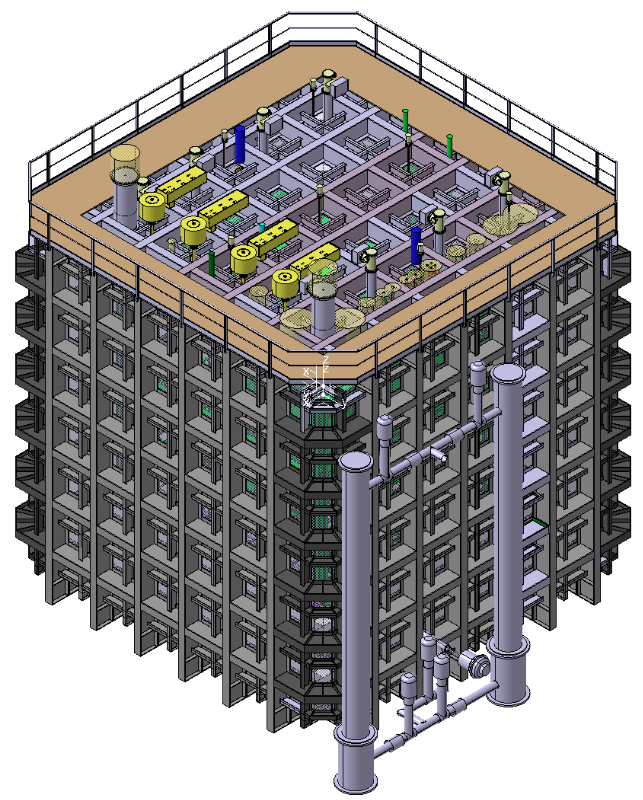
\includegraphics[width=0.8\textwidth]{protoDUNE_cryostat.png}
\end{cdrfigure}


The photon propagation is simulated using a library which contains the
probabilities of observing a photon emitted at a particular point in
space by a particular photon detector.  Here, the space is divided
into voxels a few cm on a side, and the library is indexed by photon
detector element.  For the far detector, the lookup library model may
not scale appropriately, taking too much memory to store
smoothly-varying photon visibility functions, and parameterizations
may be used for light propagating from events far from the photon
detectors, and looked up in the library for light originating from
points closer to the photon detectors.

The simulated arrival times and charge amounts on each wire, and of
each set of photons arriving at each photon detector, along with the
identity of the particles generating them, are stored in the
simulation output file for use in determining the performance of the
downstream reconstruction algorithms.  These charge depositions and
photons are inputs to the detector response functions -- the field
response and the electronics response are convoluted with the true
arrival times to make simulated waveforms.  The detector field
response functions are simulated using GARFIELD~\cite{garfield}, but
they will be validated with real data, as the simulation contains
oversimplifications, such as inadequate modeling of crosstalk between
neighboring wires.  The electronics gain is applied so that the
simulated signals match the expected responses.  Simulated noise is
then added, and the result is quantized to reproduce the behavior of a
12-bit ADC, including realistic pedestals and saturation.  A similar
process is followed to simulate the response of the photon detectors,
given the arrival times of the photons.  Functionality exists within
LArSoft to overlay Monte-Carlo-simulated particles with raw digits in
the data in order to simulate pileup of cosmics and other beam
interaction particles. The simulated raw digits are then written to
compressed ROOT files for further analysis.

LArSoft provides functionality for simulating non-LArTPC detectors as
well, labeling the additional detector elements ``auxiliary
detectors''.  These are important components for a test-beam
experiment such as ProtoDUNE-SP, as the beamline instrumentation, as
well as scintillator counters outside of the cryostat will need to be
included in the detailed simulation in order to extract precision
physics results from the experiment.  LArIAT~\cite{lariat} uses these
features of LArSoft to simulate its auxiliary detectors.